\chapter{Detailed Classes of Attacks and Vectors}

In this appendix, we will analyze several types of attacks: IP Spoofing, Packet Sniffing, Connection Hijacking, and Distributed Denial of Service (DDoS).

\raggedright
\begin{center}
    \section{IP Spoofing} 
\end{center}
A technique where an attacker alters the source IP address in a packet header to disguise their identity or impersonate another system.

\subsection{Common uses of IP spoofing}
In \textbf{Distributed Denial of Service} (DDoS) attacks, IP spoofing is employed to generate a massive amount of traffic directed at a target, using multiple spoofed IP addresses to overwhelm the target’s resources and cause a service disruption. Another use of IP spoofing is in \textbf{Man-in-the-Middle} (MITM) attacks, where attackers impersonate trusted IP addresses to intercept or alter communications between two systems, potentially reading sensitive data or injecting malicious content. Additionally, in \textbf{Session Hijacking}, attackers spoof an IP address to impersonate a legitimate device, allowing them to gain unauthorized access to an active session. Finally, in \textbf{Reflection and Amplification} attacks, attackers send spoofed requests to various servers, which then respond to the victim’s IP address, effectively flooding the victim with high volumes of traffic and causing a denial of service. 

\subsection{Mitigations for IP spoofing}
To combat IP spoofing, several strategies can be employed. \textbf{Packet filtering} is a key technique, where firewalls and routers apply rules to detect and block packets with forged IP addresses, especially through filtering at entry (ingress filtering) and exit (egress filtering) points. \textbf{Authentication mechanisms} that verify the identity of communicating devices can also enhance security, helping to prevent acceptance of spoofed packets. \textbf{Network monitoring} is crucial as well; by analyzing traffic for unusual patterns or unexpected sources, administrators can detect potential spoofing attempts early. Finally, \textbf{rate limiting} can mitigate the effects of spoofed attacks by controlling the rate of requests from individual sources, reducing the risk of overwhelming the target system.

\begin{center}
    \section{Packet Sniffing} 
\end{center}
Packet sniffing refers to the practice of eavesdropping on and analyzing network traffic. By monitoring the data packets transmitted over a network, a sniffer can capture the content of these packets, which may include sensitive information such as passwords, personal messages, or financial details.

\subsection{Common uses of Packet Sniffing}
Packet sniffing is commonly employed by network administrators for \textbf{troubleshooting} network, but it can also be misused by attackers for malicious purposes, such as \textbf{eavesdropping} or data theft. Another crucial use of packet sniffing is in security auditing. By \textbf{monitoring network} traffic, administrators can detect network vulnerabilities, unauthorized access attempts, or potential security breaches. In terms of network \textbf{performance monitoring}, packet sniffing helps track the flow of data across the network, revealing traffic patterns that might indicate performance bottlenecks or inefficiencies.

\subsection{Mitigations for Packet Sniffing}
One of the most effective ways to secure data is through \textbf{encryption}. Another important mitigation is the use of \textbf{Virtual Private Networks} (VPNs). VPNs establish a secure, encrypted tunnel for data to travel through, which protects the data from being captured by sniffers. \textbf{Network segmentation} is another crucial measure to reduce the risk of packet sniffing. By dividing a network into smaller, isolated subnets, administrators can limit the exposure of sensitive data. 

% ------

\begin{center}
    \section{Connection Hijacking} 

    (Data Spoofing)
\end{center}

An attacker takes control of an active communication session between two systems, typically by intercepting and manipulating the data exchanged. In a hijacking scenario, the attacker gains unauthorized access to the session, impersonating one of the legitimate parties to carry out malicious actions.

\subsection{Common uses of Connection Hijacking}
One common use of connection hijacking is to bypass authentication and gain unauthorized access to systems or networks. By taking \textbf{control of an established session}, attackers can avoid the need to authenticate themselves, allowing them to impersonate the victim. In some cases, attackers might hijack a connection to \textbf{launch other types of attacks}, such as man-in-the-middle (MitM) attacks. In these situations, the attacker can intercept, modify, or inject malicious data into the communication stream.

\subsection{Mitigations for Connection Hijacking}
To mitigate the risks associated with connection hijacking, strong \textbf{encryption} is essential. Another effective measure is the implementation of \textbf{session timeouts} and \textbf{re-authentication mechanisms}. By automatically terminating sessions after a period of inactivity or requiring users to re-authenticate periodically. Additionally, the use of \textbf{Multi-Factor Authentication} (MFA) significantly strengthens the security of user sessions. Even if an attacker gains control of an active session, MFA adds an extra layer of protection by requiring a second form of verification. \textbf{Secure coding} practices also play a key role in preventing session fixation attacks. Developers should implement mechanisms to generate and manage session IDs securely. 

\begin{center}
    \section{Distributed Denial of Service}
\end{center}
Multiple systems are used to flood a target network, server, or website with a massive volume of traffic, rendering it inaccessible to legitimate users. Unlike traditional denial of service (DoS) attacks, which typically come from a single source, a DDoS attack leverages multiple compromised systems, often referred to as a botnet, to amplify the scale and impact of the attack.

\subsection{Common uses of DDoS}
While DDoS attacks are primarily malicious, they can also have certain strategic uses in cybersecurity, such as testing the robustness of network defenses. Some organizations intentionally simulate DDoS attacks as part of their security assessments to understand how their infrastructure responds to high levels of traffic and to identify potential vulnerabilities in their defense mechanisms.
The most common use of DDoS attacks is to target businesses, government agencies, or other organizations in an attempt to disrupt services. These attacks can target online platforms, e-commerce sites, gaming services, financial institutions, and critical infrastructure, causing significant operational disruptions and financial losses.

\subsection{Mitigations for DDoS}
One of the most effective approaches is to deploy \textbf{traffic filtering and rate limiting systems} that can detect abnormal traffic patterns and block malicious requests before they reach the target server. Another key mitigation strategy is the use of \textbf{cloud-based DDoS protection services}, which can absorb large volumes of traffic and prevent it from overwhelming a company’s servers. \textbf{Load balancing} is another useful technique to distribute incoming traffic across multiple servers. Lastly, maintaining a \textbf{robust network architecture} with redundant systems, including backup servers and distributed content delivery networks (CDNs), can enhance resilience.



\begin{center}
    \section{Phishing}
\end{center}
Often use email or instant messaging (IM) to lure users to fake (shadow) servers with the goal of stealing sensitive information or installing malicious software. These attacks are designed to deceive users into revealing their authentication credentials or other personal data by presenting seemingly legitimate requests.

There are specialized variants of phishing that target specific individuals with tailored strategies:
\begin{itemize}
    \item Spear phishing: This variant involves crafting a more personalized message by including specific personal information, such as the user’s name, email address, department, or phone number. This makes the phishing attempt to appear more credible, increasing the likelihood that the victim will fall for the scam.
    \item Whaling: A more targeted form of phishing aimed at high-profile individuals, such as CEOs or CIOs. These attacks often involve carefully crafted messages that exploit the authority and trust associated with these VIPs.
\end{itemize}

\begin{center}
    \section{Meet-in-the-Middle}
\end{center}

The attack works by trying to find a match between intermediate ciphertexts generated by encrypting the plaintext with one key and decrypting the ciphertext with another key. By performing this process for both encryption and decryption, the attacker can reduce the complexity of breaking the encryption from a brute-force approach to a more efficient search, effectively halving the key space that needs to be searched.

\hfill

\begin{tcolorbox}[colback=lightblue, colframe=blue!50!white, title=Process Overview]
    Assumptions:
    N bit keys, plaintext \( P \), ciphertext \( C \), and keys \( K_1 \) and \( K_2 \), the relationship can be written as:
    \[
    C = \textcolor{red}{\text{enc}(K_2, \text{enc}(K_1, P))}
    \]
    
    To break this encryption, an attacker computes intermediate values:
    \[
    X_i = \textcolor{red}{\text{enc}(K_i, P)} \quad \text{and} \quad Y_j = \textcolor{red}{\text{dec}(K_j, C)}
    \]
    
    The goal is to find matching pairs such that \( X_i = Y_j \).
\end{tcolorbox}

\centering
\section{Dictionary}
\raggedright
Method used to break password hashes by systematically trying a list of precomputed potential passwords. This list, known as a dictionary, typically contains commonly used passwords or words from a specific language. It works on the assumption that users often choose weak or predictable passwords, like dictionary words, rather than random strings.

\hfill

\textbf{Application of Dictionary Attack in MS-CHAPv2}:

MS-CHAPv2 (Microsoft Challenge Handshake Authentication Protocol version 2\footnote{Security of IP networks chapter.}) is vulnerable to dictionary attacks if an attacker has access to the challenge-response pairs (from the authentication exchange) and the NT-Hash of the password.

During the MS-CHAPv2 authentication process, an attacker can intercept the challenge-response pairs (i.e., the Server Challenge (SC) and Client Challenge (CC)) exchanged between the client and the server. They can also capture the response R (which is the result of the encryption of the password hash combined with the challenge hashes).

... process ... 

The attacker then compares the computed response R with the R captured during the authentication exchange. If they match, the attacker has successfully guessed the password.

\centering
\section{Replay}
\raggedright
An attacker intercepts and retransmits a valid communication or authentication message between two parties in order to impersonate a legitimate user or gain unauthorized access to a system.

\textbf{How a Replay Attack Works:}
\begin{itemize}
    \item Capture: The attacker intercepts a legitimate message or authentication data (e.g., login credentials, session tokens, or cryptographic messages) as it travels across the network.
    \item Store: The attacker saves the intercepted data for later use.
    \item Replay: The attacker resends (replays) the intercepted message to the intended recipient or server, bypassing authentication mechanisms to gain unauthorized access.
\end{itemize}

\begin{center}
    \section{DHCP}
    (Dynamic Host Configuration Protocol - Security at Level 2)
\end{center}
Here are some types of attacks listed:
\begin{itemize}
    \item DHCP \textbf{Starvation Attack}: The attacker floods the DHCP server with many DHCP request packets, exhausting its pool of available IP addresses. Legitimate devices cannot obtain an IP address, leading to a denial-of-service (DoS).
    \item DHCP \textbf{Spoofing Attack}: The attacker impersonates a legitimate DHCP server, providing clients with malicious IP configuration.
    \item DHCP \textbf{Injection} (Malicious DHCP Options): The attacker injects malicious configuration options (e.g., false DNS servers, gateways, or proxy settings) via DHCP responses.
\end{itemize}

Best Practices for protecting Against DHCP Attacks:
\begin{itemize}
    \item Enable DHCP Snooping (an option on modern switches) to allow replies only from “trusted ports” (\textcolor{red}{requests are still broadcast}).
    \item Enable IP guard (an option on modern switches) to ensure that only legitimate traffic from authorized IP-MAC pairs is forwarded through a port.
    \item Restrict Network Access: Implement VLANs, 802.1X authentication, and port security to prevent unauthorized devices from connecting to the network.
    \item Authentication for DHCP Messages (RFC-3118) uses HMAC-MD5 (\textcolor{Blue}{authentication and integrity}) to authenticate DHCP messages. However, there are challenges with key distribution and management since it relies on a shared key.
\end{itemize}

\begin{center}
    \section{Smurfing}
\end{center}


\begin{multicols}{2}
    Type of distributed denial-of-service (DDoS) attack that exploits the Internet Control Message Protocol (ICMP) and the IP broadcast feature to amplify traffic and overwhelm a target system or network. 

\columnbreak

    \begin{figure}[H]
        \centering
        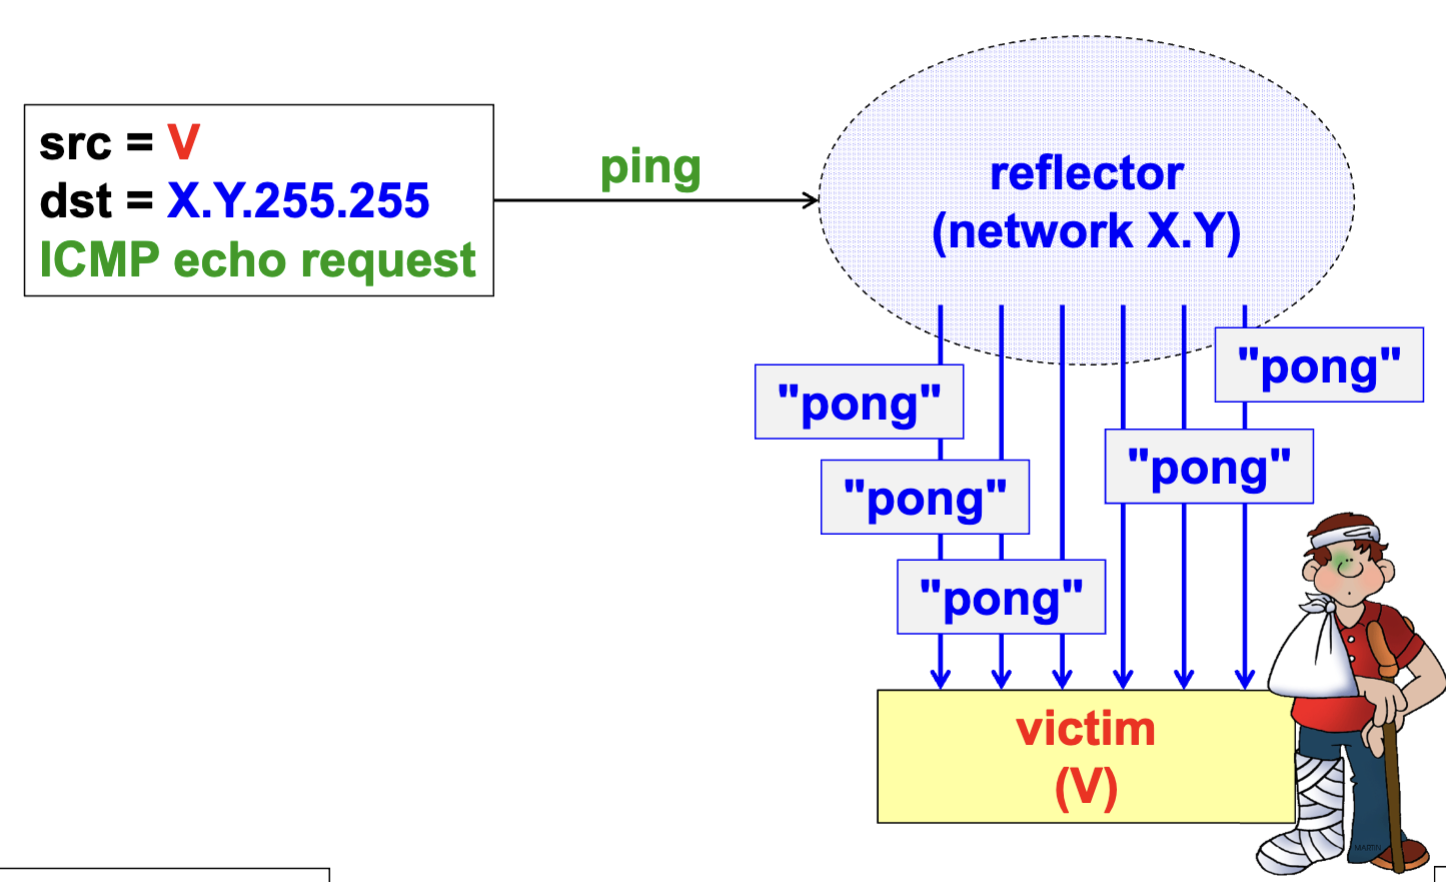
\includegraphics[width=0.5\linewidth]{Images/NetSec/smurfing.png}
        \caption{Smurfing Attack example.}
    \end{figure}
\end{multicols}

Here’s how it works:







% --------











\section{Attack Vectors}

\begin{table}[H]
    \centering
    \begin{tabular}{|p{3cm}|p{12cm}|}\hline
    \rowcolor{blue!10}
    \textbf{Vector} 
        & \textbf{Description}  
    \\ \hline

    Trojan
        & Appears as legitimate software or a harmless file to deceive users into installing it. Contains a dangerous payload and is often used to create a Man At The End or a Man In The Browser.
    \\ \hline
    
    Virus
        & Attaches itself to legitimate files or programs and spreads by infecting other files on a system. Is propagated by humans (often involuntarily).
    \\ \hline

    Worm
        & Self-replicating malware that spreads across networks without requiring user intervention. Unlike a virus, a worm does not need to attach itself to a file or program.
    \\ \hline

    Backdoor
        & Unauthorized access point, it allows an attacker to remotely control the system or retrieve sensitive information without the knowledge of the legitimate users or administrators.
    \\ \hline

    Rootkit
        & Designed to gain unauthorized access to a system and maintain privileged control (root access) while hiding its presence from users and security software.
    \\ \hline

    Potentially Unwanted Applications (PUAs)
        & Software programs that are not inherently malicious but may negatively impact a user’s system or experience. They often include programs like adware, toolbars, or system optimizers that may be bundled with other software. While PUAs typically don’t cause direct harm like viruses or malware, they can degrade system performance, display excessive ads, or compromise privacy by collecting personal data without clear consent. 
    \\ \hline

    Ransomware 
        & Encrypts a user’s files or locks them out of their system, rendering the data inaccessible. The attacker then demands a ransom.
    \\ \hline



\end{tabular}
\caption{Attack Vectors}
\label{tab:attackVectors}
\end{table}